\chapter{Data Preparation and Model Training}


Ideally, the ATN should be trained with paired waveforms ($X, X'$) where $Y=Y'$ for each pair. In reality, it is impossible to collect such a paired dataset: we can simulate $\mathcal{T}_{Source}$ from an arbitrary $\mathcal{D}_{Source}$, but it is impossible to collect $\mathcal{T}_{Target}$ so that $\mathcal{D}_{Source} = \mathcal{D}_{Target}$ without knowing the exact form of $P(X'|Y')$. Therefore, the training has to be conducted on $\mathcal{T}_{Source}$ and $\mathcal{T}_{Target}$ given that $\mathcal{D}_{Source} \neq \mathcal{D}_{Target}$. The CycleGAN framework~\cite{CycleGAN} allows us to train ATN on such an unpaired dataset. We first construct two networks an ATN~ $\Lambda$ and an Inverse ATN $\bar{\Lambda}$, both with PU-Net structure. We then construct two discriminator networks $\delta_{S}$ and $\delta_{T}$ for the source and target waveforms, respectively. 

Combining all these, we obtain the Cyclic Positional U-Net~(CPU-Net) for Ad-hoc pulse shape simulation. The trained CPU-Net produces both an ATN and an IATN, translating waveforms between the source and target domain. The ATN is the primary interest of this work, but the IATN can also be adopted to boost the physical analysis.


\label{chap:training}
The shape of the detector pulses is affected by many parameters, including particle energy, interaction position, charge cloud size, and so on. The relationship between the location of energy deposition and the resulting detector pulse is illustrated in Figure~\ref{fig:eng_dep_sim}. The left panel shows the interaction locations of particles within the detector for selected events. Event 3 and Event 4 are effectively single-sited, as the energy depositions occur very close to each other. In Event 1, the energy depositions result in two primary sites, giving rise to a two-sited pulse. Event 2 features a trace of energy deposition localized to three regions, classifying it as a three-sited event. 

\begin{figure}[htb!]
  %[trim={left bottom right top},clip]
    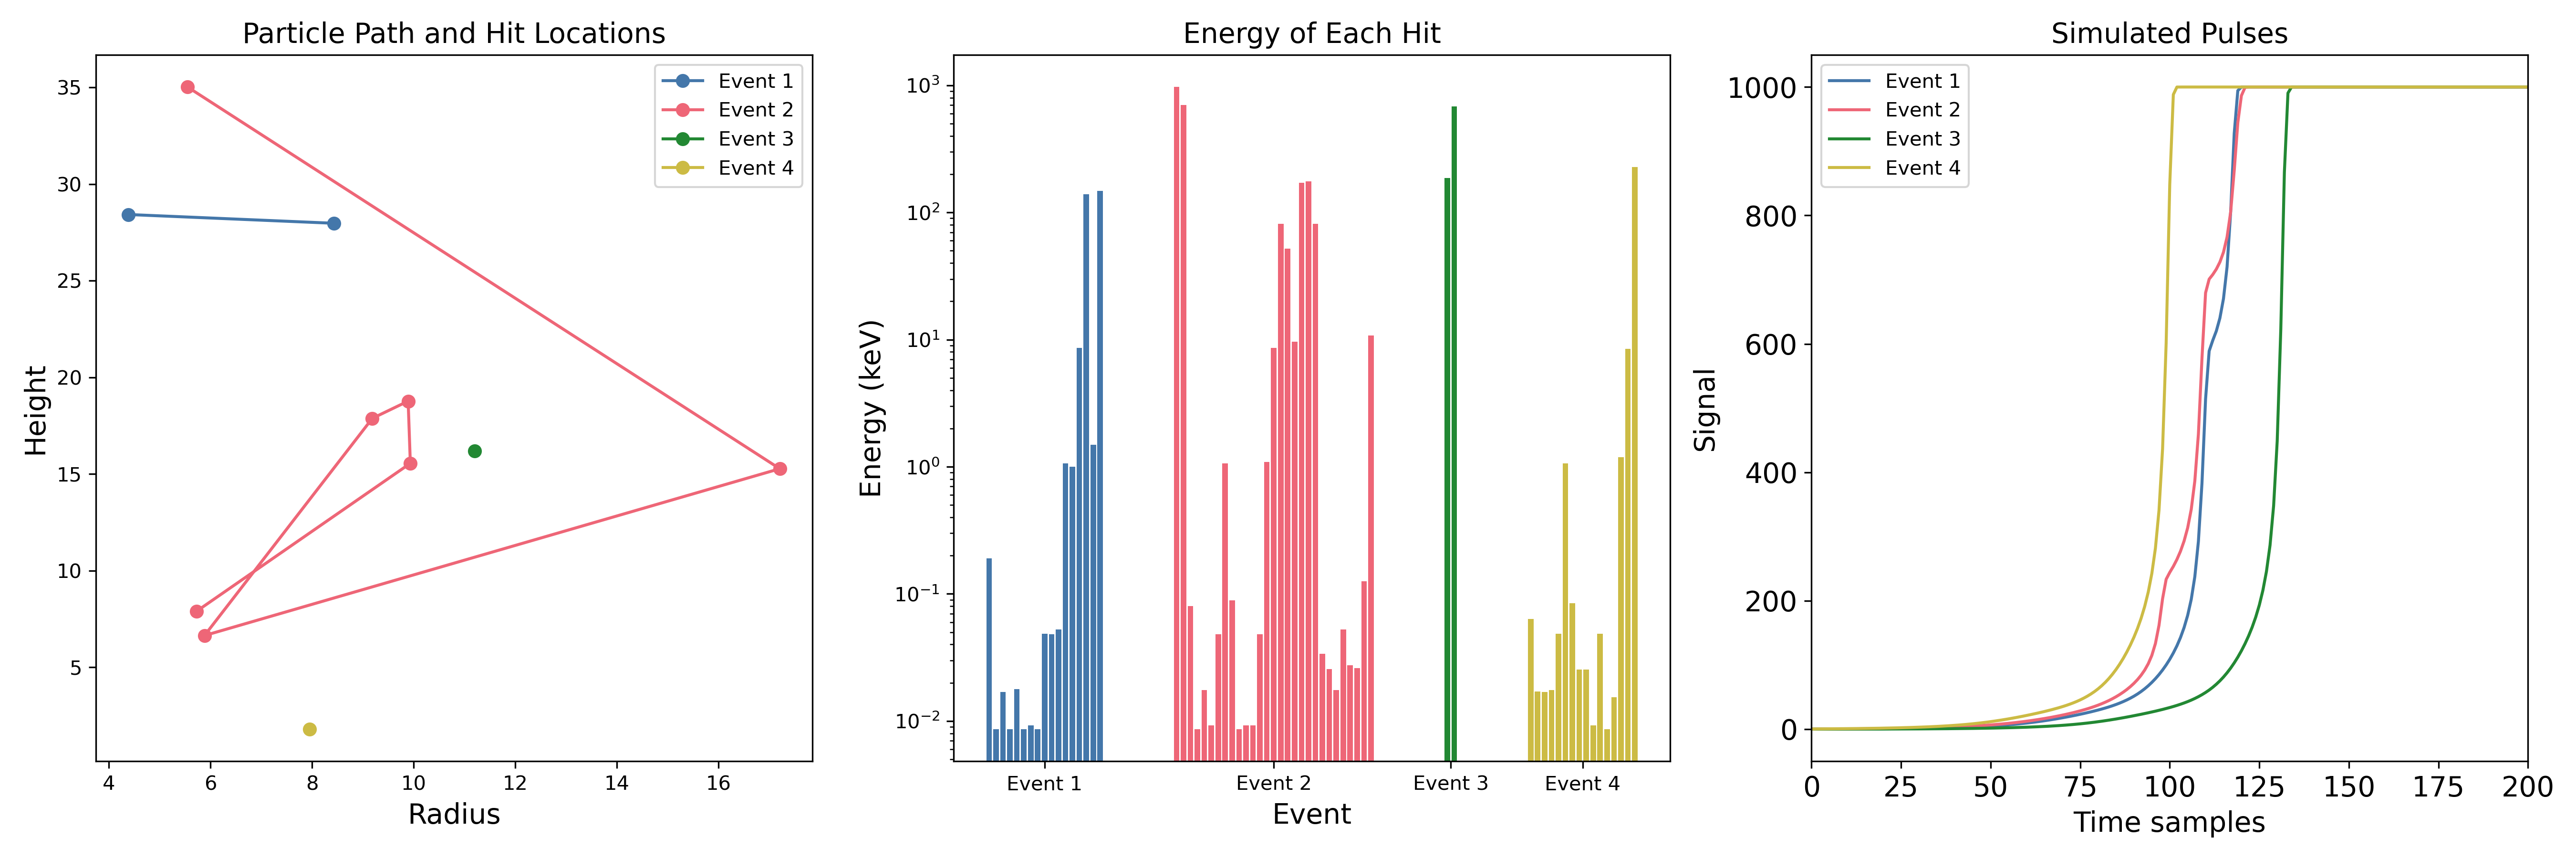
\includegraphics[width=0.99\linewidth,trim={1pc 0pc 1pc 0pc},clip]{ch7/figs/hit_sims.png}
    \caption{(Left) Hit locations for each event. (Right) Energy-weighted pulses for the corresponding events. Hits produced using \texttt{Geant4} simulations and pulses generated using \texttt{siggen} software.}
   \label{fig:eng_dep_sim}
\end{figure}

\begin{figure}[htb!]
    % \hspace{0.05\linewidth}
    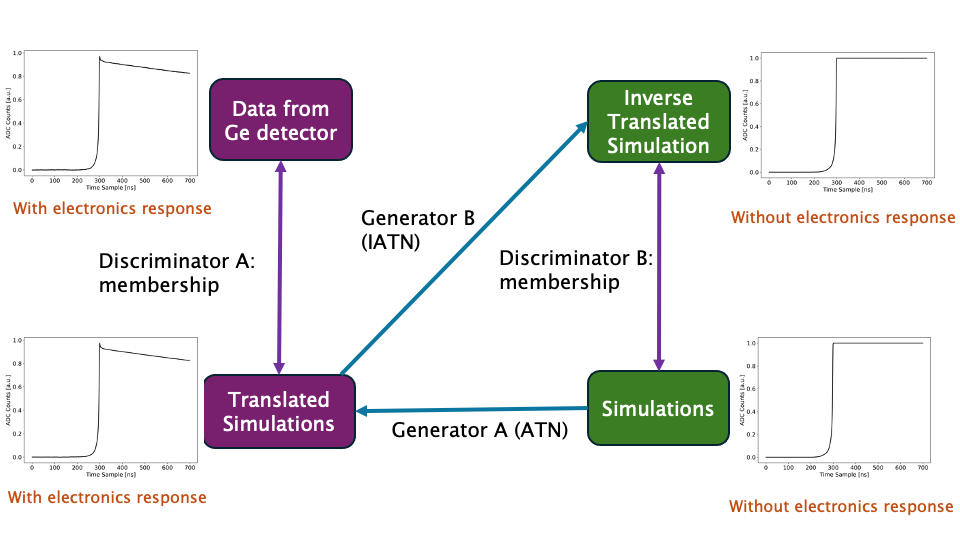
\includegraphics[width=0.99\linewidth]{ch7/figs/cycle_gan_training.png}
    \caption{Cycle-consistent adversarial training with PU-Net as the Ad-hoc Translation Network~(ATN) and Inverse Ad-hoc Translation Network~(IATN). The red oval region represents simulated pulses in $\mathcal{T}_{Source}$, and the blue oval region represents detector pulses in $\mathcal{T}_{Target}$.}
   \label{fig:network_training}
\end{figure}

\begin{table}%[ht!]
\centering
\renewcommand{\arraystretch}{1.5} % Adjust row height for readability
\setlength{\tabcolsep}{2.0pt} % Adjust column spacing
\begin{tabular}{|p{0.18\linewidth}|p{0.39\linewidth}|p{0.22\linewidth}|p{0.15\linewidth}|}
\hline
Loss                & Calculation                             & Type of Loss                                  & Optimizer   \\ \hline
Identity Losses    & Data - ATN(Data)                                & \multirow{3}{=}{Custom L1 Loss} & \multirow{8}{=}{Optimizer 1} \\
                             & Sim - IATN(Data)                                 &                                                       &                       \\ \cline{1-3}
Cycle Losses        & Data – ATN(IATN(Data))                         & \multirow{3}{=}{Custom L1 Loss} &                       \\
                             & Sim – IATN(ATN(Sim))                          &                                                       &                       \\ \cline{1-3}
Generator Losses    & Disc B (IATN(Data))                              & \multirow{2}{=}{Binary Cross Entropy}                &                       \\
                             & Disc A (ATN(Sim))                              &                                                       &                       \\ \hline
Discriminator A     & {[Disc A(Data) - 1]} + {[Disc A(Sim) - 0]}        &  Binary Cross Entropy                                & Optimizers 2 \\ \hline
 Discriminator B    & {[Disc B(Sim) - 1]} + {[Disc B(Data) - 0]}        &   Binary Cross Entropy                                &   Optimizers 3             \\ \hline
\end{tabular}
\caption{Overview of Loss Calculations, Loss Types, and Optimizers.}
\label{ch8_tab_loss_summary}
\end{table}




% \section{Training and Hyperparameter Search}\label{subapp:hyperparam}
% Two major pulse categories that low-background HPGe experiments seek to distinguish are single-site~(SS) and multi-site~(MS) events. When a physical event deposits all its energy in a single location in a detector, a SS pulse with a single sharply-rising step is produced. Conversely, a MS pulse with multiple steps is produced if energy is deposited at multiple locations within the crystal. SS and MS pulses of the same total energy can be efficiently distinguished by the maximal current amplitude reconstruction parameter $I_{max}$.
\section{Data selection (Kevin)}

In addition to prominent source peaks, a germanium gamma-ray spectrum is characterized by three main interaction processes: photoelectric absorption, Compton scattering, and pair production. At higher energies (~5–10 MeV), pair production dominates. In this process, the incident photon generates an electron-positron pair. The electron is collected by the detector, while the positron quickly annihilates, producing two additional gamma-ray photons. If all secondary gamma rays are fully absorbed within the detector, their combined energy yields a characterized peak in the energy spectrum, the Full Energy Peak (FEP).



If one of the annihilation gamma rays leaves the detector without depositing its energy, the spectrum shows a Single Escape Peak (SEP). This scenario results in a multisite (MS) event because the signal comprises two distinct interactions within the detector: the collection of the pair-produced electron and the absorption of one of the two gamma rays. If both gamma rays escape the detector without interaction, a double escape peak (DEP) is observed. This situation corresponds to a single site (SS) event since the only interaction that contributes to the signal is the collection of the pair-produced electron.


% Rare events neutrinoless double-beta decay are typically single sited events. Low-background HPGe experiments thus seeks to distinguish between single site from multi site events. SS and MS pulses of the same total energy can be efficiently distinguished by the maximal current amplitude parameter $I_{max}$ \cite{mjd_psd}. For a given event energy, SS pulses have faster $I_{max}$ than MS pulses. This difference arises because SS events generate a localized energy deposition that leads to a sharp current peak as the charge is collected. MS events involve interactions occurring at multiple points within the detector, result in a more spread-out energy deposition and thus lead to multiple current peaks, contributing to a slower current compared to single site (SS) events.

Tl-208 is part of the decay chain of $^{228}$Th, and produces an FEP at $2614.53$ keV. Given the mass of the electron is $511$ keV, the SEP peak occurs at $2103.53$ keV and the DEP peak at $1592.53$ keV. The FEP peak is an excellent region for training given its abundance and the fact that it contains a mixture of single and multi-site events. SEP and DEP can then be used as a validation data set, evaluating the model's response to multi-site and single-site events, respectively.

The LEGEND collaboration characterizes newly produced HPGe detectors at Oak Ridge National Laboratory (ORNL). We used data from a LEGEND Inverted-Coaxial Point-Contact (ICPC) detector, V06643A, manufactured by ORTEC and measured at ORNL. The detector was enclosed in a “PopTop” configuration, surrounded by lead shielding, and placed in a concrete alcove to reduce external backgrounds. We used the data from a run with a Thorium-232 source placed on top of the detector. The data was digitized using a FlashCam digitizer. The pygama package was used to convert FlashCam output to LEGEND LH5-format HDF5 files and to calibrate event energy from ADC units into keV\cite{pygama}. The energy was then corrected for charge trapping corrections. Fig. \ref{fig:eng_spec} left panel shows the final energy spectrum from the detector. 
%The dspeed package provides optimized numba based processors for digit signal processing \cite{dspeed}. The current was calculated using dspeed by running a derivative filter, up-sampling the output, running a multi window moving average and taking maximum value.

\begin{figure}%[htb!]
  %[trim={left bottom right top},clip]
    \centering
    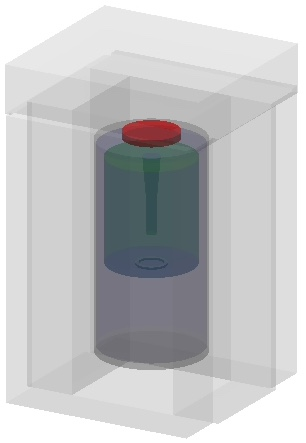
\includegraphics[width=0.4\linewidth]{ch7/figs/shielding.jpeg}
    \caption{The simulation geometry of the ORNL characterization setup, showing the detector in green, the source in red, the aluminum holder in light blue, and the lead shielding in light grey.}
   \label{fig:g4simple_setup}
\end{figure}


\begin{figure}%[htb!]
  %[trim={left bottom right top},clip]
    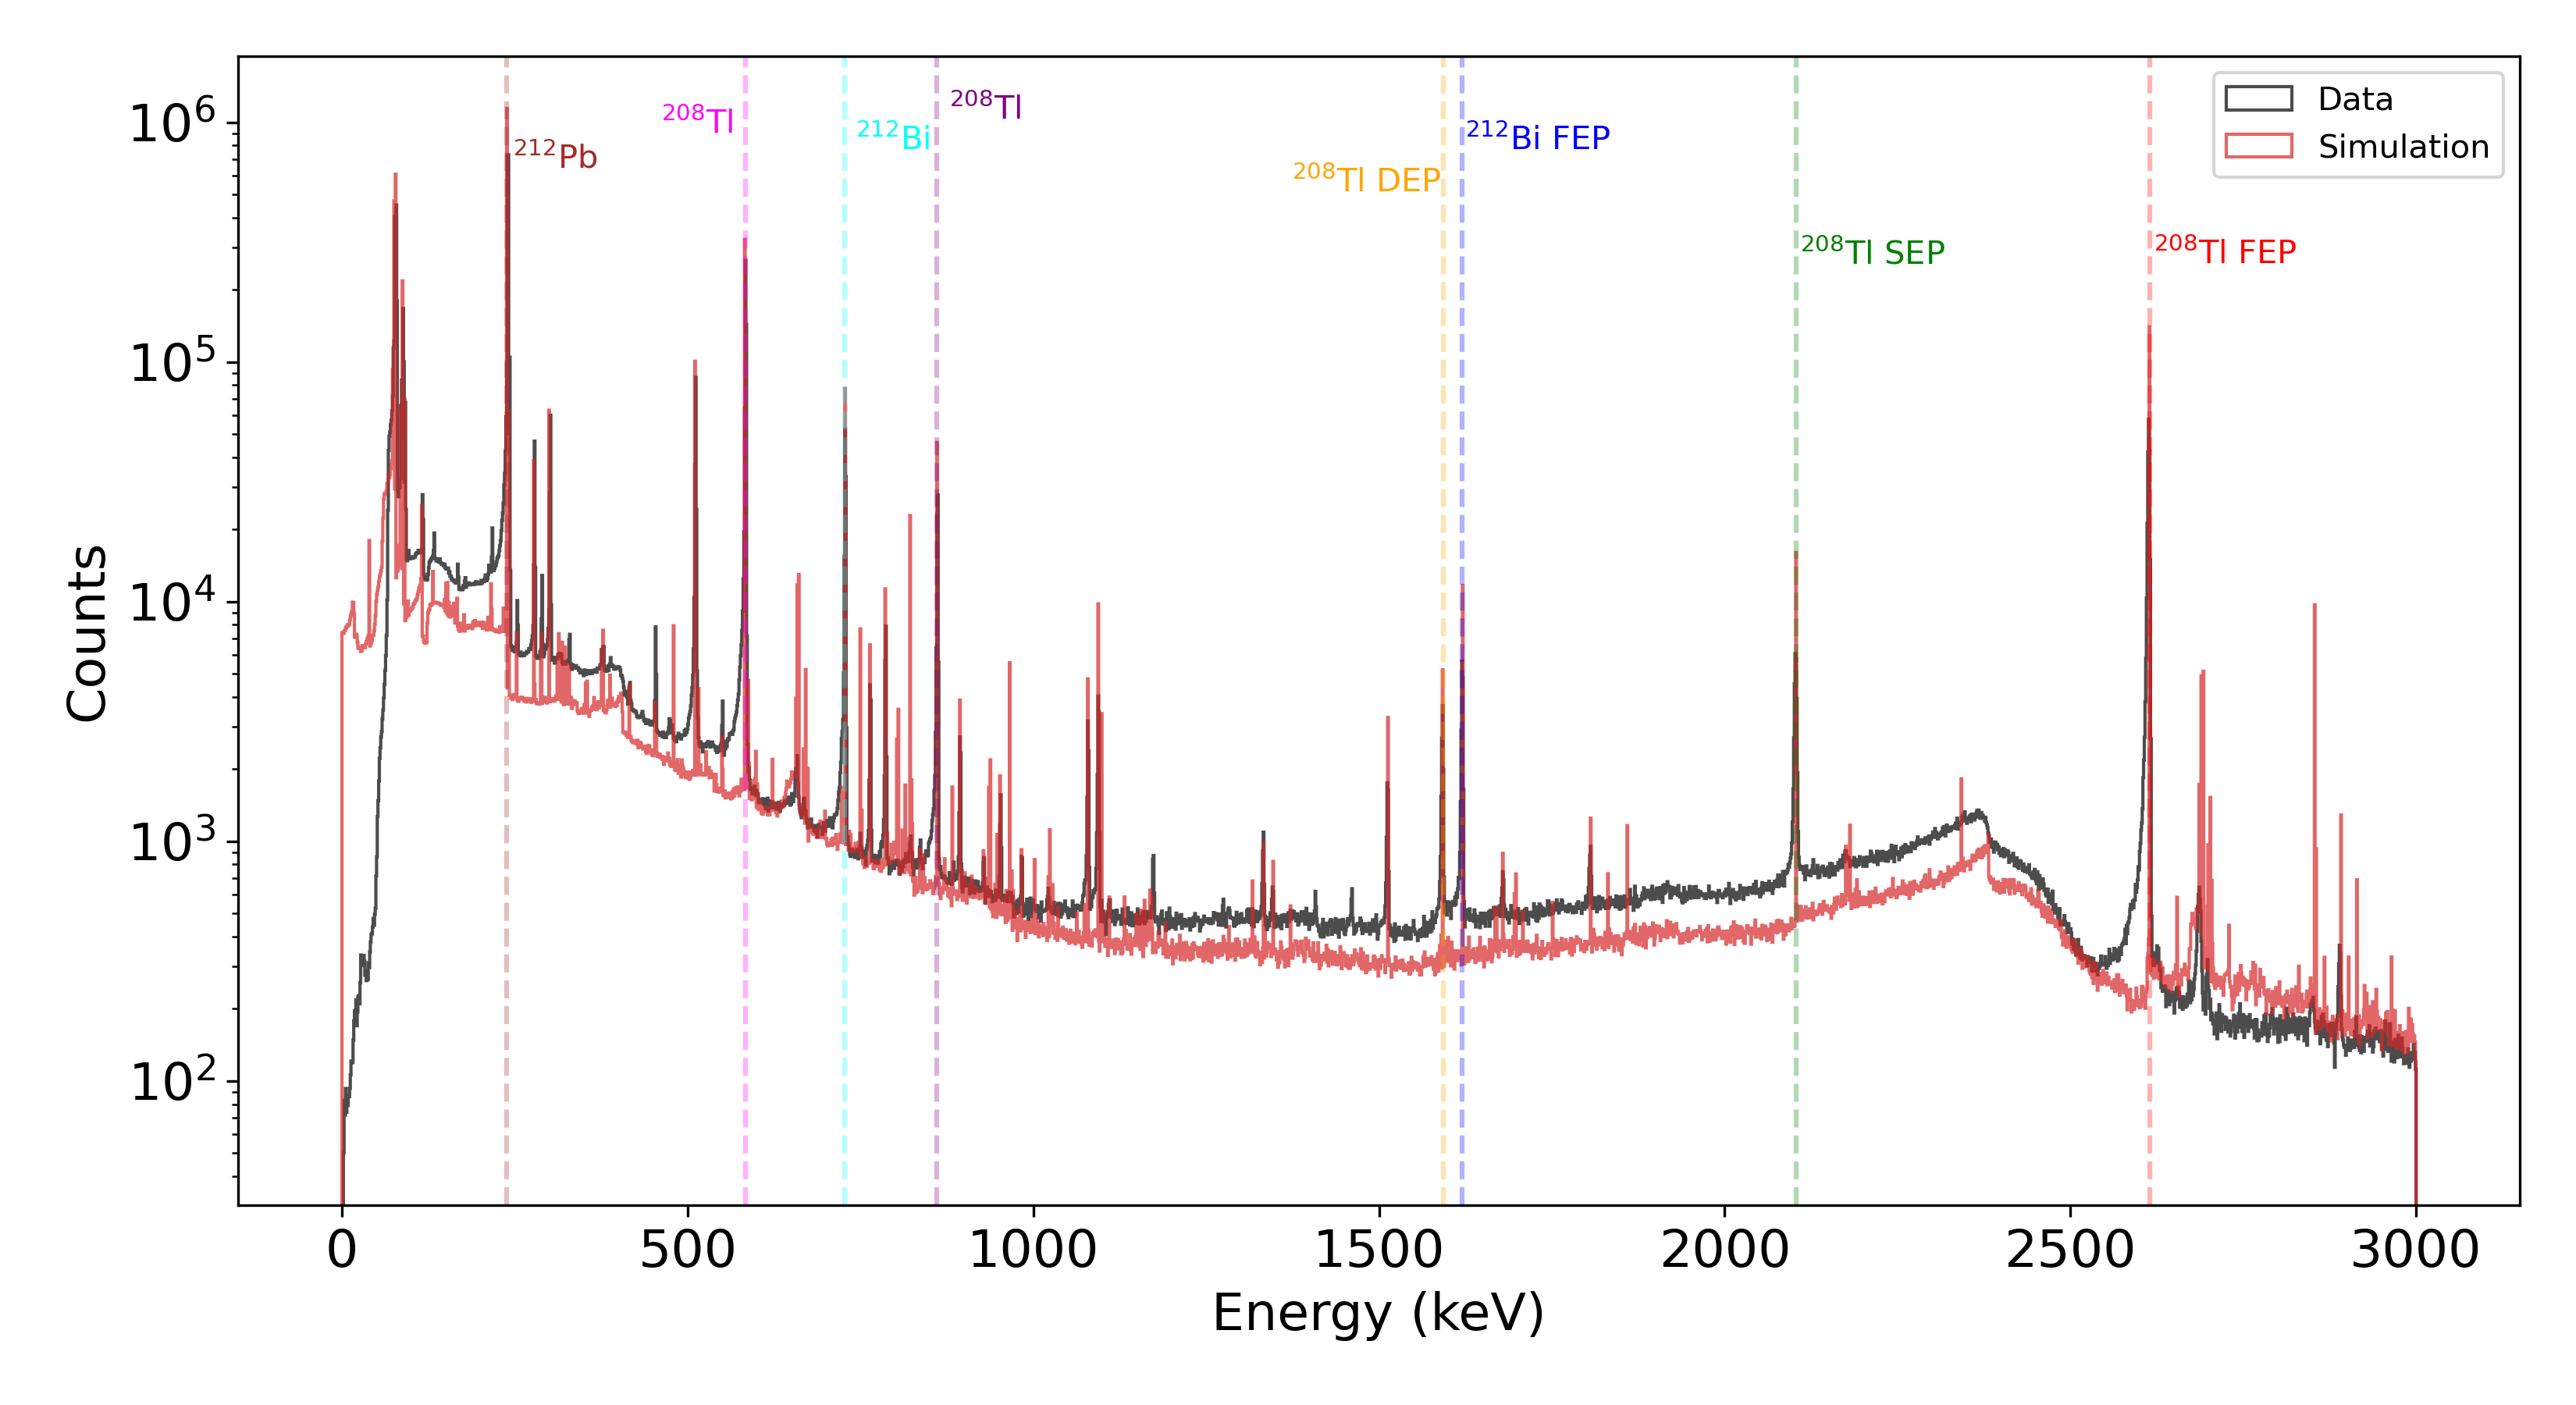
\includegraphics[width=0.99\linewidth,trim={1pc 0pc 1pc 0pc},clip]{ch7/figs/energy_spectrum_comparison.png}
    \caption{Measured energy spectrum from a $^{228}$Th source compared to the Monte Carlo simulation results. Key peaks from $^{228}$Th source are labeled.}
   \label{fig:eng_spec}
\end{figure}



- Normalization
- Alignment

\section{Simulations (Kevin)}
Geant4 is a Monte Carlo-based toolkit that can simulate the passage of particles through matter. We designed a Geant4 setup geometry to simulate the hits of the setup of ORNL characterization shown in Fig. \ref{fig:eng_spec} This includes a Germanium detector, a radioactive source, Aluminum PopTop cryostat holder, surrounded by lead shielding. We simulated 100 million $^{228}$Th decay events originating from the source and recorded their energy depositions within the germanium detector. Given the location of energy deposition inside the detector, we used Siggen simulations to generate pulses for hits in a 1 keV window around DEP, SEP and FEP. Pulses for the same event were stacked together and normalized by event hit energies, thus producing multi-site events.

\section{Post processing and Network Training}
Each raw pulse~(simulated pulses or data pulse) is first normalized and aligned by the time needed to reach $99\%$ of their maximum value. The pulses are padded to ensure there are 400 samples on both sides of $99\%$ rise time. The tail slope $\tau$ is calculated by the slope of a linear fit of the logarithm of the last 200 pulse samples. Events with poor fit quality $\chi^2$ or anomalous $\tau$ are used to identify pile-up pulses and exclude them from the training.

% In addition, we apply one-hot encoding and embedding before feeding normalized pulses into the RNN discriminator. The one-hot encoding is conducted through multiplying WF$_{norm}$ by 500 and rounding to the nearest integer. Then a PyTorch embedding layer is used to convert each one-hot encoding vector to an \textit{m}-dimensional embedding vector, where \textit{m} is the embedding dimension and one of the model hyperparameters.

The training and validation of CPU-Net are conducted in PyTorch~\cite{pytorch}. When training the network, a simulated pulse $X$ is first fed to $\Lambda$ to produce a translated pulse $\Lambda(X)$, then an adversarial training with $\delta_{T}$ is performed: $\delta_{T}$ attempts to distinguish $\Lambda(X)$ from $\mathcal{X}'$ while $\Lambda$ attempts to ``fool'' $\delta_{T}$. Then $\Lambda(X)$ is fed to $\bar{\Lambda}$ to translate back to $\mathcal{X}$ space by $\bar{\Lambda}(\Lambda(\mathcal{X}))$. A second discriminator $\delta_{S}$ attempts to distinguish $\bar{\Lambda}(\Lambda(\mathcal{X}))$ from $\mathcal{X}$ while $\bar{\Lambda}$ attempts to ``fool'' $\delta_{S}$. The $\mathcal{X}\rightarrow{}\Lambda(\mathcal{X})\rightarrow{}\bar{\Lambda}(\Lambda(\mathcal{X}))$ translation path is denoted by the red arrows in the right-side panel of Figure~\ref{fig:network_training}. The same process is performed in the other direction, starting with the detector pulse, $\mathcal{X}'\rightarrow{}\bar{\Lambda}(\mathcal{X}')\rightarrow{}\Lambda(\bar{\Lambda}(\mathcal{X}'))$ is denoted by blue arrows in the same figure.  

$L_{\mathrm{Identity}}$ ensures that the ATN preserves its shape when an actual detector pulse $X'$ is fed into $\Lambda$, shown in Eq. \ref{eq:loss_ided}. The cycle-consistent loss in Eq. \ref{eq:loss_cyc} ensures the circular translation path preserves the original pulse shape, and the GAN loss Eq. \ref{eq:loss_gan} calculates the loss associated with ``fooling'' the discriminator. A specialized L1 loss is used for $L_{\mathrm{Identity}}$, $L_{\mathrm{Cycle}}$, $L_{\mathrm{Advesarial}}$ that emphasizes different parts of the pulse by assigning them varying weights. It's particularly designed to give more importance to the rising and falling edges of the pulse, which are critical for accurate pulse shape analysis. Binary Cross-Entropy Loss is used for the discriminator $\delta_{T}$.

\begin{equation}\label{eq:loss_ided}
    L_{\mathrm{Identity}} = |X' - \Lambda(X')|
\end{equation}
\begin{equation}\label{eq:loss_cyc}
    L_{\mathrm{Cycle}} = |X - \bar{\Lambda}(\Lambda(X))|
\end{equation}
\begin{equation}\label{eq:loss_gan}
    L_{\mathrm{Adversarial}} = E_{\mathcal{X'}}\log(\delta(X')) - E_{\Lambda(\mathcal{X})}\log(1 - \delta(\Lambda(X)))
\end{equation}

An additional three complementary losses are defined for the detector pulse translation path. Therefore, a total of six losses are optimized simultaneously for the generators and two for the discriminators. AdamW~\cite{adam_w_paper} optimizers are used for all losses. We trained the CPU-Net on 110,000 FEP waveforms. A linear learning rate decay begins at iteration 1000 and reaches zero at the final iteration.

To prevent overfitting during training, weight decay is applied to the optimizers so that it penalizes the large weights and encourages generalization. Gradient clipping is applied, limiting the norm of gradients during training and preventing exploding gradients, particularly in layers of the U-Net.

It was found that the discriminator typically overpowers the generator since the generator has a more complex task of generating pulses while maintaining the cycle and identity consistency, and also fooling the discriminator. To balance this, we introduce a hyperparameter for the number of intervals after which the discriminator is updated. This allowed the generator enough steps to adapt to changes in the discriminator without destabilizing the adversarial process.


\label{chap:cpu-net_result}


\begin{table}[ht!]
\centering
\renewcommand{\arraystretch}{1.5} % Adjust row height for readability
\setlength{\tabcolsep}{4pt} % Adjust column spacing
\begin{tabular}{|p{0.23\linewidth}|p{0.12\linewidth}|p{0.55\linewidth}|}
\hline
\textbf{Hyperparameter}       & \textbf{Value} & \textbf{Description} \\ \hline
\texttt{batch\_size}          & 32             & Number of pulses used in one training iteration \\ \hline
\texttt{baseline\_len}        & 200            & Number of samples assigned to the baseline portion of the waveform. \\ \hline
\texttt{rising\_edge\_len}    & 250            & Number of samples assigned to the rising edge of the waveform. \\ \hline
\texttt{tail\_len}            & 350            & Number of samples assigned to the RC decay tail of the waveform. \\ \hline
\texttt{baseline\_weight}     & 3.0            & Weight given to the baseline portion of the waveform in the loss function. \\ \hline
\texttt{ris\_edge\_weight}    & 10.0           & Weight given to the rising edge portion of the waveform in the loss function. \\ \hline
\texttt{tail\_weight}         & 7.0            & Weight given to the RC decay tail portion of the waveform in the loss function. \\ \hline
\texttt{iters}                & 7000           & Maximum number of iterations for training. \\ \hline
\texttt{decay}                & 1000           & Iteration at which learning rate starts to decay. \\ \hline
\texttt{lrate\_gen}           & $1 \times 10^{-3}$ & Learning rate for the generator networks. \\ \hline
\texttt{lrate\_disc}          & $1 \times 10^{-3}$ & Learning rate for the discriminator networks. \\ \hline
\texttt{cyc\_loss\_weight}    & 20             & Weight of the cycle consistency losses.  \\ \hline
\texttt{iden\_loss\_weight}   & 5              & Weight of the identity loss. \\ \hline
\texttt{gan\_loss\_weight}    & 9              & Weight of the generator loss. \\ \hline
\texttt{max\_grad\_norm}      & 100            & Maximum gradient norm for gradient clipping. \\ \hline
\texttt{w\_decay}             & $1 \times 10^{-4}$ & Weight decay in the optimizers. \\ \hline
\texttt{n\_disc\_iters}       & 30             & Number of iterations after which the discriminators are updated. \\ \hline
\end{tabular}
\caption{Hyperparameters used for CPU-Net training.}
\label{tab:hyperparameters}
\end{table}


Table \ref{tab:hyperparameters} shows the hyperparameters used in the training. Together these parameters enable price fine-tuning CPU-Net training to get the right balance during training. A single training takes about 1 GPU hour on a NVIDIA A100 GPU.